\section{Generowanie i przechowywanie danych}
Generowanie danych jest oparte o informacje uzyskiwaną z 
czujników pomiarowych:
\begin{itemize}
  \item \texttt{DHT11} - czujnik temperatury i wilgotności,
  \item \texttt{BH1750} - czujnik natężenia światła.
\end{itemize}
Zakresy pomiarowe czujniku \texttt{DHT11} stanowią pewne ograniczenie
na jego zastosowanie:
\begin{itemize}
  \item Temperatura -- [0,50] $\pm 2^\circ$ o rozdzielczości $1^\circ$,
  \item wilgotność -- [20,90]\% \texttt{RH} - wilgotność względna. 
    Jest to stosunek rzeczywistej wilgoci w powietrzu do maksymalnej jej ilości, 
    którą może utrzymać powietrze w danej temperaturze.
    Rozdzielczość -- $1\%$.
\end{itemize}
Z powodu powyższych ograniczeń, dany czujnik można stosować w warunkach, które
nie wymagają większej precyzji, na przykład -- pomieszczenia biurowe.

Czujnik natężenia światła posiada szeroki zakres pomiarowy -- $[1,65535] lx$,
z rozdzielczością 1 lub 4 $lx$ w zależności od wybranego trybu pracy. 
W danej implementacji została wybrana rozdzielczość w 1 $lx$.

\subsection{Przechowywanie danych}
Ze względu na małą ilość zbieranych danych, 3 wartości typu \texttt{int}, w zakresie
[0, 65535], przez długi okres czasowy (do 150 dni, przy okresie pomiarowym 1 minuta), 
został zdefiniowany plik w formacie \texttt{csv}.

Dane rozwiązanie zostało przyjęte ze względu na 
przechowywane dane, łatwość w użyciu, w porównaniu do baz danych, oraz 
brak nadmiarowych informacji -- plik przechowuje tylko te dane, 
które zostały do niego zapisane.

\begin{lstlisting}[frame=single, basicstyle=\ttfamily\small,
caption={Definicja pliku \texttt{csv} z przykładowymi danymi}]
Temperature,Light,Humidity
25,380,57
\end{lstlisting}

\subsection{Podłączenie czujników}
Czujniki zostały podłączone do wejść \texttt{GPIO} platformy
\textsl{Raspberry Pi 3B+} w poniższy sposób:
\begin{figure}[h!]
  \centering
  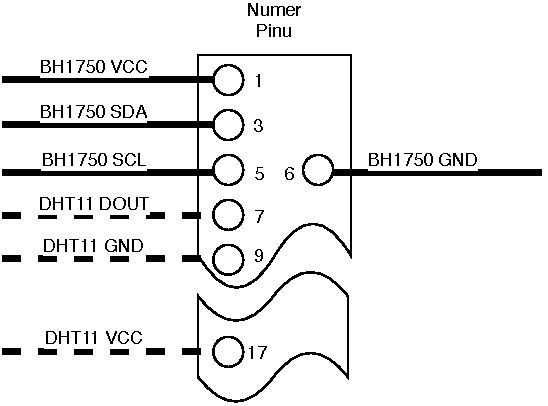
\includegraphics[scale=1]{pins.pdf}
  \caption{Połączenie pinów czujników z wejściami \texttt{GPIO}}
\end{figure}

W celu komunikacji i uzyskania danych z czujników zostały użyte moduły:
\begin{itemize}
  \item \texttt{smbus}
  \item \texttt{Adafruit-DHT}
\end{itemize}

\newpage
Dla uzyskiwania danych co określony czas (domyślne ustawione na 1 minutę) został
napisany proces, który pobiera dane z czujników i zapisuje je do pliku oraz 
proces monitorujący:
\begin{lstlisting}[frame=single, basicstyle=\ttfamily\small, language=python,
caption={Definicja objektu nadzorującego proces zbierający dane}]
class Sensors():
    def __init__(self):
        self.thread = None
        self.runner = runner.Runner(60)
        self.is_running = threading.Event()
\end{lstlisting}

\begin{lstlisting}[frame=single, basicstyle=\ttfamily\small, language=python,
caption={Inicjalizacja procesu zbierającego dane}]
def reset_sensors(self, _sleep=60):
        """
        Funciton initialize the thread
        which will collect data from sensors
        based on provieded 'sleep' timeout
        Timeout = [60,3600]
        """
        if self.thread is None:
            self.is_running.clear()
            self.runner.set_sleep(_sleep)
            self.thread = threading.Thread(target=self.runner.launch,
					   args=(self.is_running,))
            self.thread.start()
	    ...
\end{lstlisting}
\begin{lstlisting}[frame=single, basicstyle=\ttfamily\small, language=python,
caption={Definicja procesu zbierającego dane}]
class Runner():
    def __init__(self, _sleep):
        self.sleep = _sleep
        self.data = data.Sensors_data()
        self.bus = smbus.SMBus(1)
        self.light = bh1750.BH1750(self.bus)
        self.dht = dht11.DHT()
\end{lstlisting}
\begin{lstlisting}[frame=single, basicstyle=\ttfamily\small, language=python,
caption={Zbiór i zapis danych}]
 def launch(self, is_running):
        while not is_running.is_set():
            _humid, _temp  = self.dht.read()
            if _humid == -1:
                time.sleep(self.sleep)
            else:
                _light  = int(self.light.measure_high_res())
                self.data.save_average([_temp, _light, _humid])
                time.sleep(self.sleep)
\end{lstlisting}
